\section{Performance}
A brief overview of the performance section.

\subsection{Performance of the Transport Subsystem}
\label{sec::performance::transport}
% Written by Rob
We received discouraging, but explainable, results in our scaling test.  For the
brief overview, refer to figure \ref{fig::performance::transport::procs-time}.
This graph represents a reduced search-space trial on 4, 8, 16, 32, 64, and 128
processes respectively.

\begin{figure}[htp]
\begin{centering}
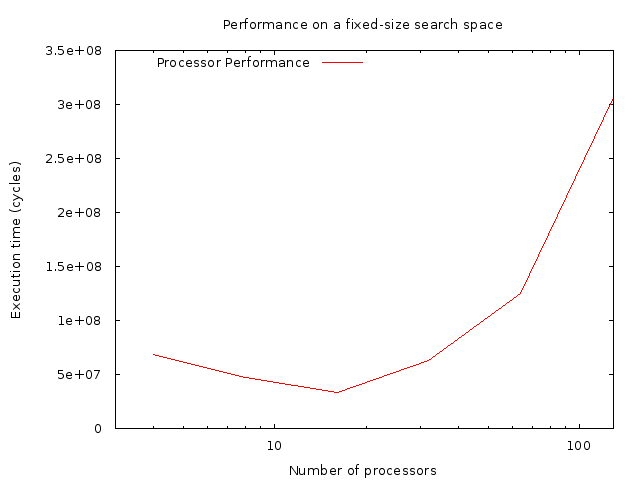
\includegraphics[height=.25\textheight]{strong-scaling.png}
\label{fig::performance::transport::procs-time}
\end{centering}
\end{figure}

Up until 16 processors we see the run time decrease; after that point it grows
to greater than that required for a sequential implementation.  There are two
very compelling reasons as to why this phenomenon occurs.

First and foremost, we noticed that our implementation was especially
susceptible to OS jitter in our development environment.  Our results mirrored
those shown in \cite{petrini}; that is, on a 4-way system, performance on up to
3 cores showed no scaling issues.  Running on 4 cores showed the effects of OS
jitter as detailed in \cite{petrini}.  We were able to offset these effects by
tuning the ratio of generation and hashing to MPI overhead.

When run on an MPI shared memory implementation, the vast majority of execution
time of our program is spent in system calls.  To us this indicated that the
ratio of hashing to communication was low.  Increasing the amount of messages
generated and hashed before each MPI\_Allreduce managed to decrease the overhead
of the system calls.  Increasing it too much had the opposite effect and all
gains were lost.

For our strong scaling trial we used the optimum ratio computed for three
processors on a shared memory MPI implementation.  Resource limits on the CCNI
prevented us from performing the same trial on 128 processors to determine the
optimum ratio for that system.  We expect that doing so would allow us to
significantly increase our performance for runs above 16 cores.

\subsection{Performance of the Storage Subsystem}
% Written by Alex
A tree-based structure was decided upon due to simplicity and the nature of the data.
Given that hashes are randomly distributed an unoptimized tree should yield better than 
average results regardless, reaching very close to log(n) memory access without amortization.
The main downside is about 50\% overhead on top of the existing 16 bytes of data. An additional
8 bytes are required, 4 bytes for the offset of each the left and right nodes in the tree
based structure. The total file size for $2^{33}$ hashes grows from 128GB to 192GB.

Before scaling naive implementations were built and tested. The first method uses
standard POSIX file operations. Unfortunately this results in
severely low throughput. A meager 10,000 hashes required upwards of 7s seconds
for insertions. Colliding all of these hashes took less time with 2s. 

\begin{figure} 
        \caption{Tests performed on a core-2-duo}
\begin{tabular}{lll}
Number of Hashes    &    All New Hashes   &  All Colliding\\
10000           &        7.334          &     2.307 \\
20000           &       14.323          &     4.908\\
30000           &       22.910 & \\
40000           &       31.792 & \\
\end{tabular}
\end{figure}

The moral of the story when doing file access is to not do file access. As seen in the
figure, linearly longer time is required per 10000 hashes. Completely colliding collisions
were not performed for 30000 and 40000 hashes. 

The best case is to use more memory and cache data before doing writes. Since 64-bit linux
machines were targeted, other POSIX features were available. And luckily,
POSIX compliant operating systems provides mechanisms to already do all of this.
Files can be directly mapped into memory using the mmap system call. Behind the
scenes the operating system takes care of swapping pages of memory in and out
from the disk to main memory, caching write-backs, and other possible optimizations.


\begin{figure} 
        \caption{File size = 48 MB  (2097152 hashes maximum capacity / file); tests run on 4-way AMD Opteron 848 using ext3}
\begin{tabular}{lll}
Number of Hashes &    All New Hashes    &    All Colliding\\
1000000         &      2.782    &            2.185 \\
2000000          &     4.749     &           3.275 \\
2100000           &    4.872      &          \\
2200000            &   39.553      &         \\
\end{tabular}
\end{figure}


\begin{figure} 
        \caption{File size = 960 MB  (4194304 hashes maximum capacity / file); tests run on 4-way AMD Opteron 848 using ext3}
\begin{tabular}{lllll}
Nodes &       2 & 4 & 6 & 8 \\
1000000 &       1.359 & 1.806 & 2.606 & 3.228 \\
2000000 &  3.099 & 3.916 & 5.557 & 7.315 \\
4000000 &  7.142 & 10.052 & 13.651 & 16.251 \\
8000000 &  16.443 & 19.484 & 30.689 & 35.662 \\
10000000 & 22.064 & 24.725 & 39.787 & 47.716 \\ 
20000000 & 50.498 & 52.026 & 90.325 & 105.694 \\
40000000 & 125.898 & 143.518 & 245.808 & 277.117\\
\end{tabular}
\end{figure}

The result was a 300-fold speed improvement from skipping file I/O except when absolutely
necessary. 

Storage is distributed by assigning a segment of the search space to each node. 
Multiple files per node were briefly tested. It was discovered that switching between files
severely damages performance. When the number of hashes grows to 220000, 
a second file is mapped into into memory. The storage model plays hot potato with the first
and second files, reloading 48 MB each time. This is unacceptable. 

The conclusion is that each node should maintain only one file which can be mapped once at
the program start and thereafter incur very little performance loss. The file size required
per node is around 1GB. To show scaling, the multithreaded tests were performed using a file size of
960MB which can store approximately 40,000,000 hashes. The results show that the tree-based
structure works adequately with a large filesize and scales for each additional thread. The largest
number of hashes stored was 160 Million which took 4.5 minutes and 7.15GB of data for a throughput
of 27 MB/s. 

\begin{figure} 
        \caption{64 bit hash}
\begin{tabular}{lll}
Nodes    &       total hashes /node       &     total size /node \\ 
16    &    $2^{29}$         &                 12   GB \\ 
64    &    $2^{27}$         &                  3   GB \\
128   &    $2^{26}$         &                 1.5  GB \\
256   &    $2^{25}$         &                 0.75 GB \\
\end{tabular}
\end{figure}

To successfully perform a collision attack on a 64-bit hash the current storage model requires 
between 128 and 256 nodes with between 1-1.5 GB of memory per node.

At the time of publishing the test was not be completed. The main conclusion from the performance
tests of the storage model is that with enough nodes the collision is feasible. From a practical
stand point, today standard hashes are 128-bits, and future cryptographic hashes are 256-bits minimum.
Performing a birthday attack on a 128-bit hash is equivalent to searching the whole 64-bit space, 
which can not be possible without massive memory improvements in computer architecture.


\subsection{Performance of Mock Hashing}
\label{sec::performance::mock}
% Written by John

The mock hashing was benchmarked so that it could be compared to DES speeds.
On an IBM T60p laptop running 2.33 GHz Core2 CPU, over 280 million hashes per
second were observed from
a dummy hash algorithm.  This was done so that we would have data equivilent
to what DES would give for testing, but allow tests to run at faster speeds,
allowing us to predict if a DES attack was feasible by scaling the time 
required.

\subsection{Performance DES Hashing}
\label{sec::performance::des}
% Written by John

The DES implementation we used is based on GNU Privary Gaurd (GnuPG).
Several implemenations were tried, including custom ones.  However,
this implmeenation was found to be the fastest and more portable.
OpenSSL contained an x86 assembly implementation, but time did not
permit extracing this for use in our implementation.  GnuPG was portable,
easy to integrate, and easy to improve.

The following describes the metrics of computing single DES hashes.
In actual birthday attack analysis, we would be required to compute
multiple DES hashes per message in order to form a hash.  Although
no standardized method exists, it is common practice to run DES
on a 64 bit block and then use the resultant data as a key to the
next block.  This would mean that the DES hashing would be an order 
of magnitude slower than the DES encryption.  However, we would
only have to hash up to the section were the document was changed.
This would mean that if we modified the last line of the document,
it could still be very long and we would not incur any signifigant
performance penalties. 

A number of improvements have been made to the GnuPG implemenation.
First, all error checking has been removed.  The code will no longer
check for things like weak keys and bad pointers.  Next, all return
values have been removed when uncessary.  A lot of this stems from the
removal of the error checking which would usually be propogated as a
return code.  A number of functions are now inlined.  This will eliminate
several function calls per round.  However, the feature that sped hashing
up the most was to turn variables passed in functions into global variables.
The most important of these is the structure that contains the keys.
This improvement alone raised hashing speeds by over three times.
The initial implementation tests showed 1.3 million DES hashes per second.
After tuning the algorithm, 4.9 million hashes per second were observed.

The DES APIs exposed are independent of the underlying implementations.
They were, however, optomized to work with the GnuPG implemtnation on
a 64 bit machine.  Internally the generic DES code calls inlined
implementation specific DES functions.  The fastest way to compute DES
is to call a set key function and then the last key set is assumed for 
later encrypt functions. However, tests showed little difference in performance
between the 32 and 64 bit versions.  The 32 bit version ran at 4.9 million
hashes per second on a 2.33 GHz Intel Core2.  The 64 bit version ran at
5.3 million hashes per second on a 2.66GHz Intel Xeon system.  This
difference in performance is about what could be expected for the 
clock speed increase and does not show any improvement for using the 
64 bit machine.  This is attributed to the GnuPG implementation being
improved to use global char arrays such that passing parameters is no
longer an issue.  Had char ararys been still passed instead of 64 bit
integers, the 64 bit implemntations probably would have shown performance.

There are several known fast hardware DES implementations.
The Electronic Frontier Foundation DES Cracker was produced in 1998 by the
Electronic Frontier Foundation to counter the government's claims about
how prohivitivly expensive and slow an attack on DES would be\cite{eff}.
The machine
consists of 1,500 Depp Crack application specific integrated circuits (ASIC)
attached to a personal computer.  The chips work by guessing at which keys are
not correct and more or less performs a brute force search.  Their attack
is slightly different as they are trying to find the key, and we have a known
key and are trying to forge the data.  However, they are still very related
and make a good comparison.  They had a peak rate of 88 billion hashes per 
second.  They were successful in their project as they were able to solve 
several RSA Security challenges.

After the EFF DES Cracker, COPACOBANA (Cost-Optimized Paralell COde Breaker)
was built using Xilinx Spartan FPGAs\cite{copacobana}.  
It has comparable speed to the EFF cracker.
Although it was designed for DES, it is highly reconfigurable, so could be
used for a wide variety of parallel applications.  It has the key advantage
that while the EFF machine was bulit for \$210,000 and additional machines
could be produced for \$120,000, COPACOBANA can be built for \$5,000.
This leads to a much higher scale of hardware attack. 

